\documentclass{beamer}
\graphicspath{{./figures/}} 
\mode<presentation>
{
  \usetheme{default} 
  \usecolortheme{default}
  \usefonttheme{default}
  \setbeamertemplate{navigation symbols}{}
  \setbeamertemplate{caption}[numbered]
} 

\usepackage[portuguese]{babel}
\usepackage[utf8]{inputenc}
\usepackage{graphicx}
\usepackage{subfigure}
\usepackage{booktabs}

\title[]{Estudo de estruturas de dados eficientes para abordar o 
problema de otimização U-Curve}
\author{Gustavo Estrela, Marcelo Reis}
\institute{Universidade de São Paulo e Instituto Butantan}
\date{\today}

\begin{document}

\begin{frame}
  \titlepage
\end{frame}

\section{Objetivo}
\begin{frame}{Objetivo}
    \begin{itemize}
        \item{Estudo do Algoritmo U-Curve Search (UCS) 
            \protect\cite{msreis thesis}}
        \item{Estudo de diagramas de decisão binária reduzidas e
            ordenadas (ROBDDs)}
        \item{Implementação de um novo algoritmo para solucionar o 
            problema U-Curve que use ROBDDs para controlar o espaço de
            busca.}
    \end{itemize}
\end{frame}

\section{Algoritmo UCS}
\begin{frame}{UCS}
    \begin{itemize}
        \item{Resumo da dinâmica:}
        \begin{itemize}
            \item{Escolha uma direção para percorrer o reticulado 
                booleano;}
            \item{Escolhe um elemento $X$ minimal (ou maximal) do
                espaço de busca;}
            \item{Percorre elementos a partir $X$ como um DFS.}
        \end{itemize}
        \item{Tem como vantagem computar poucas vezes a função de 
            custo}
        \item{Seu problema de escalabilidade se deve em grande parte
            a utilização de listas duplamente encadeadas para armazenar
            restrições ao espaço de busca.}
    \end{itemize}
\end{frame}

\section{ROBDDs}
\begin{frame}{ROBDDs}
    \begin{itemize} 
        \item{Pode responder rapidamente se um elemento está ou não
            no espaço de busca.}
        \item{Operações de atualização podem ser caras.}
        \item{O seu tamanho depende da ordem das variáveis.}
        
    \end{itemize}
\end{frame}

\begin{frame}{ROBDDs}
\begin{figure}[ht!]
        \centering 
            \subfigure[] {\scalebox{0.3}{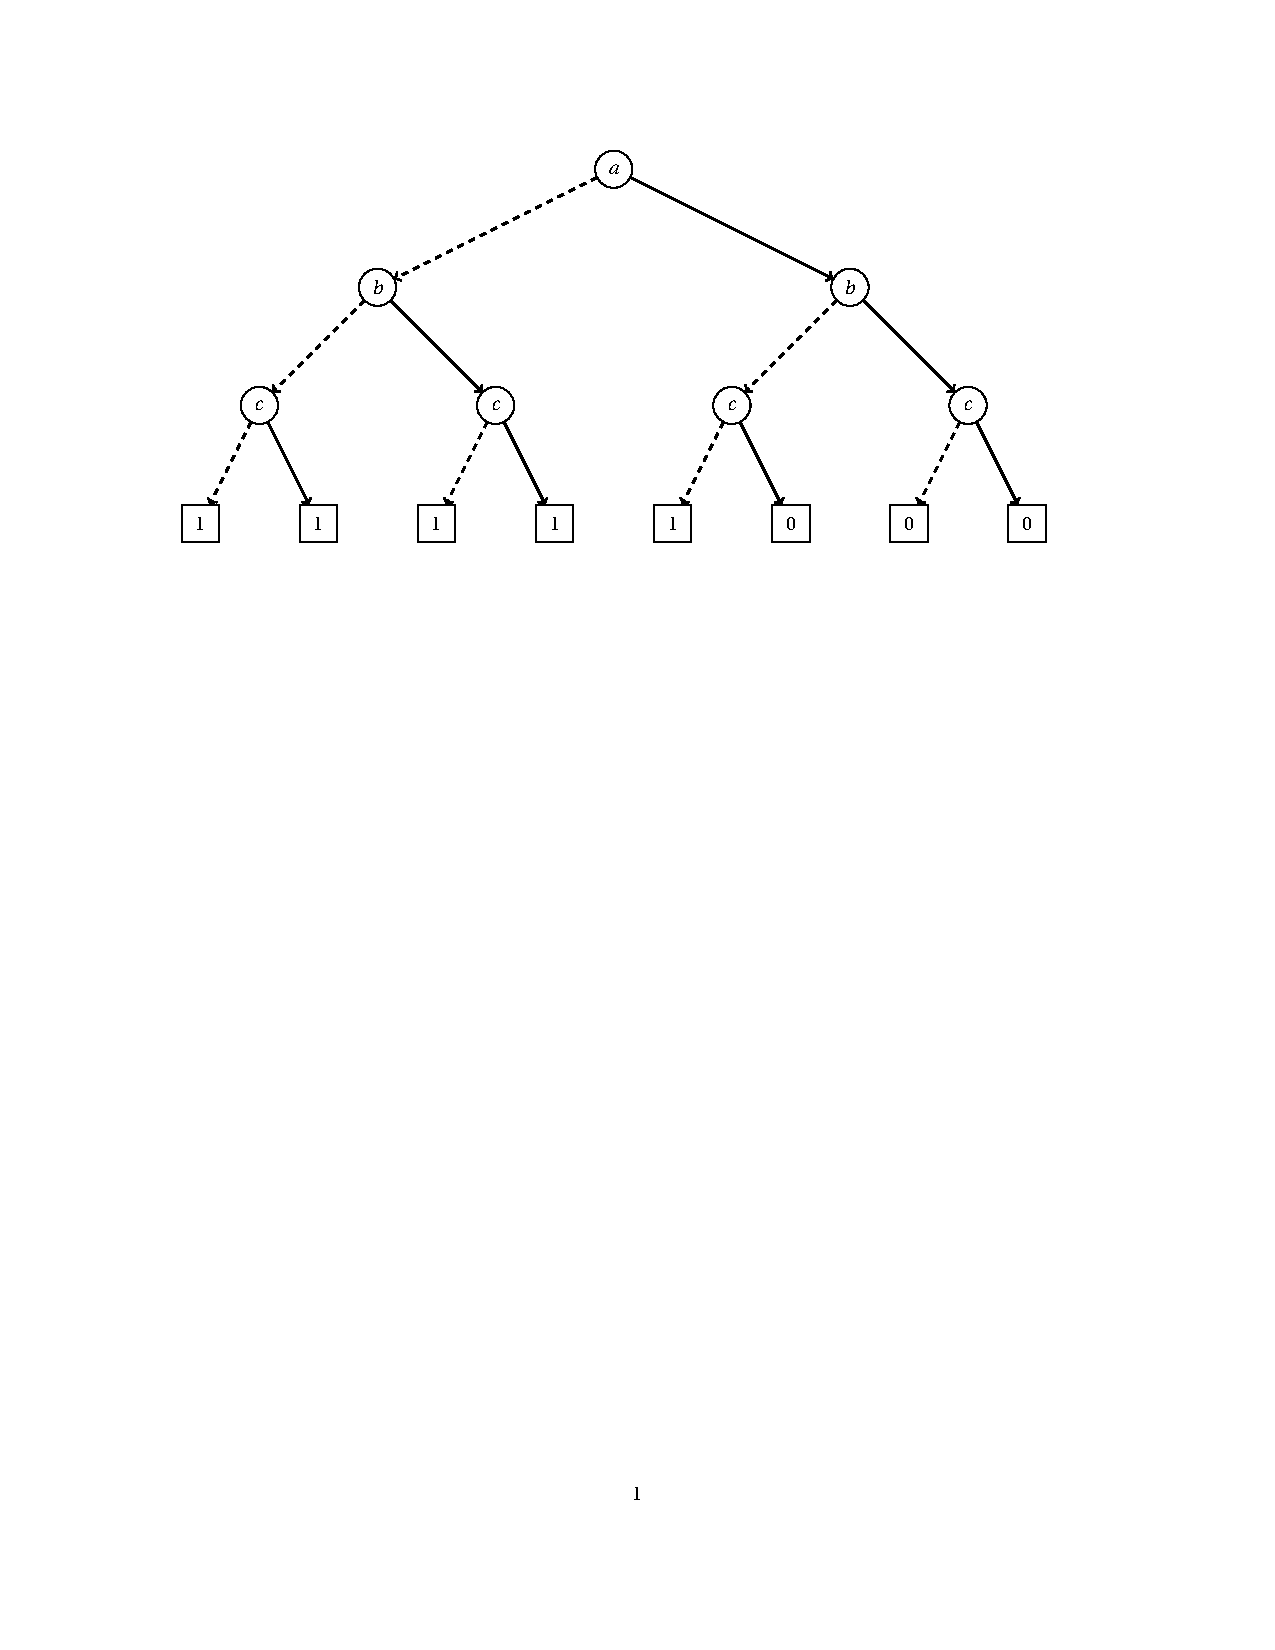
\includegraphics[
                trim=2cm 17.5cm 2cm 2cm, clip=true]{Binary_tree_3.pdf}}
                \label{fig:ROBDDs:A}}  
            \begin{tabular}{c c}
            \subfigure[] {\scalebox{0.25}{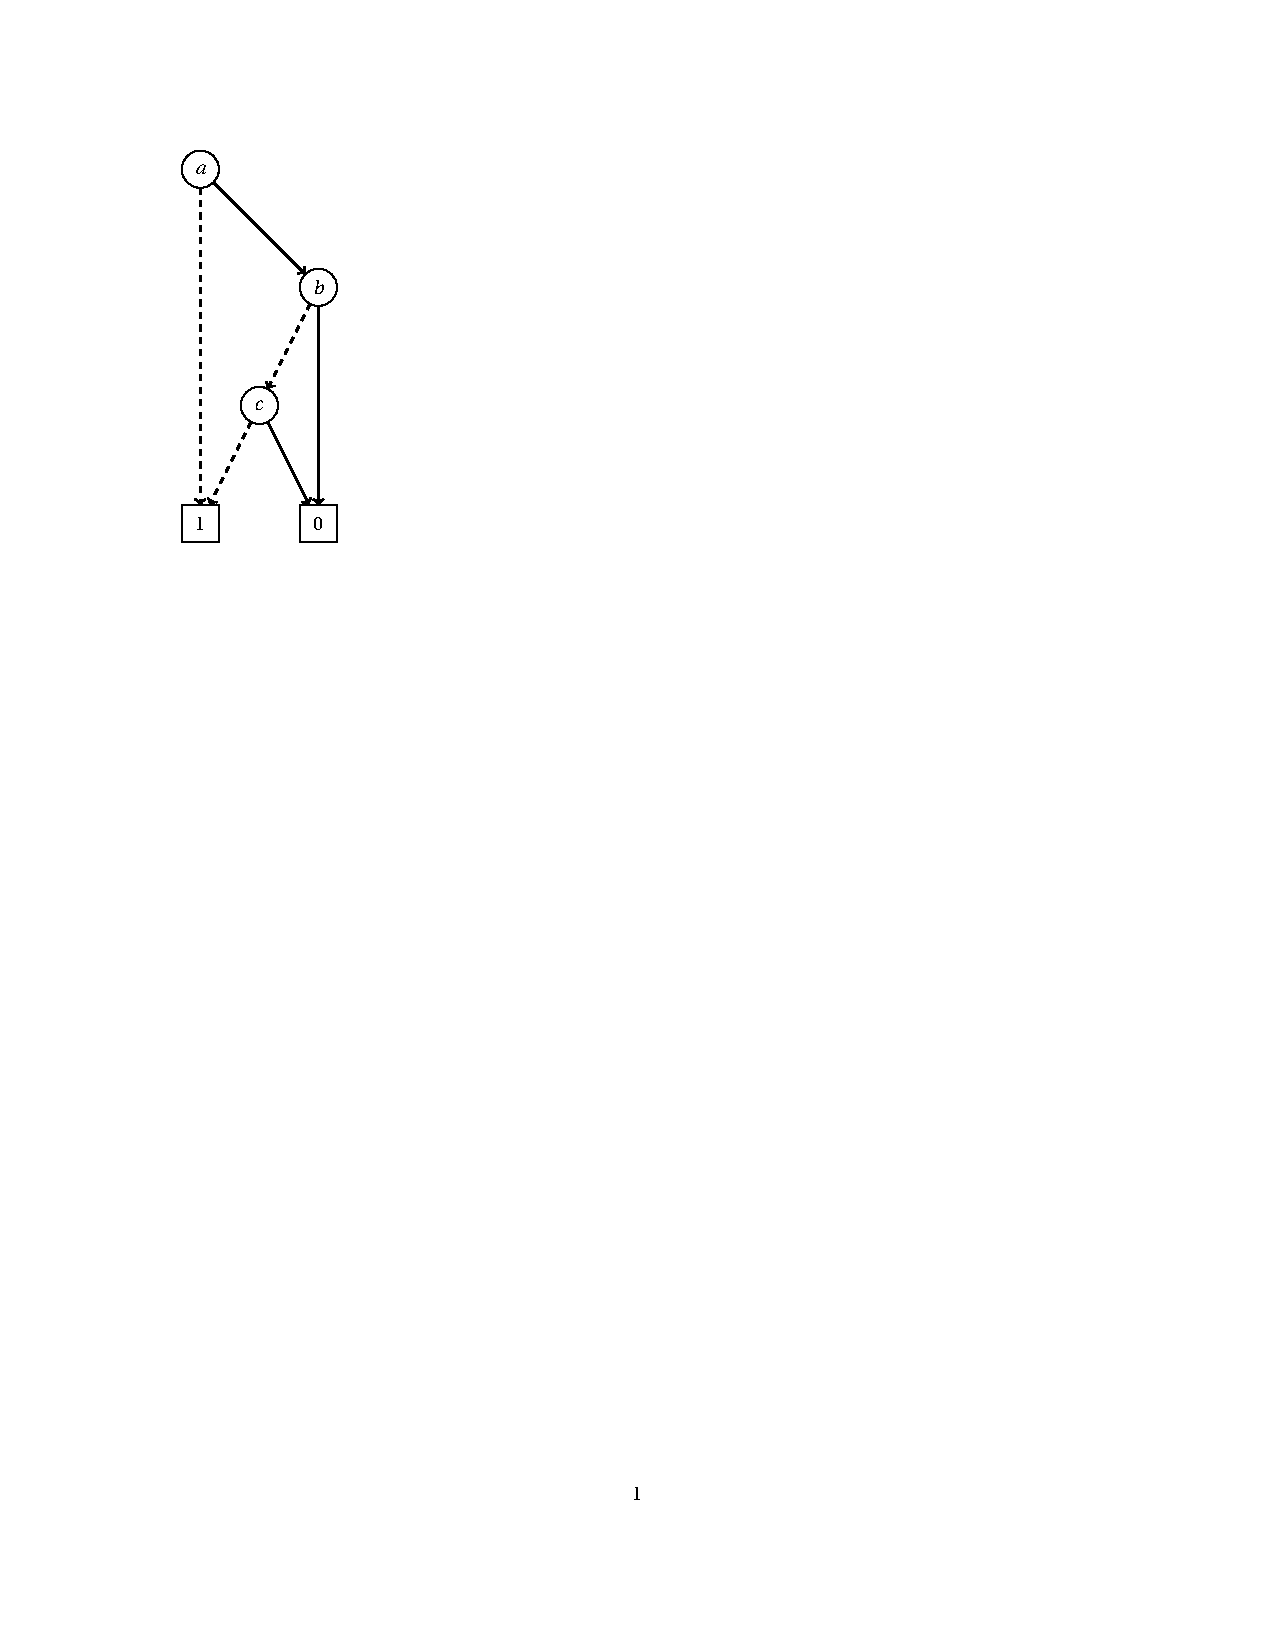
\includegraphics[
                trim=0cm 17.5cm 12.2cm 2cm, clip=true]{ROBDD_good.pdf}}
                \label{fig:ROBDDs:B}}  
  &
            \subfigure[] {\scalebox{0.25}{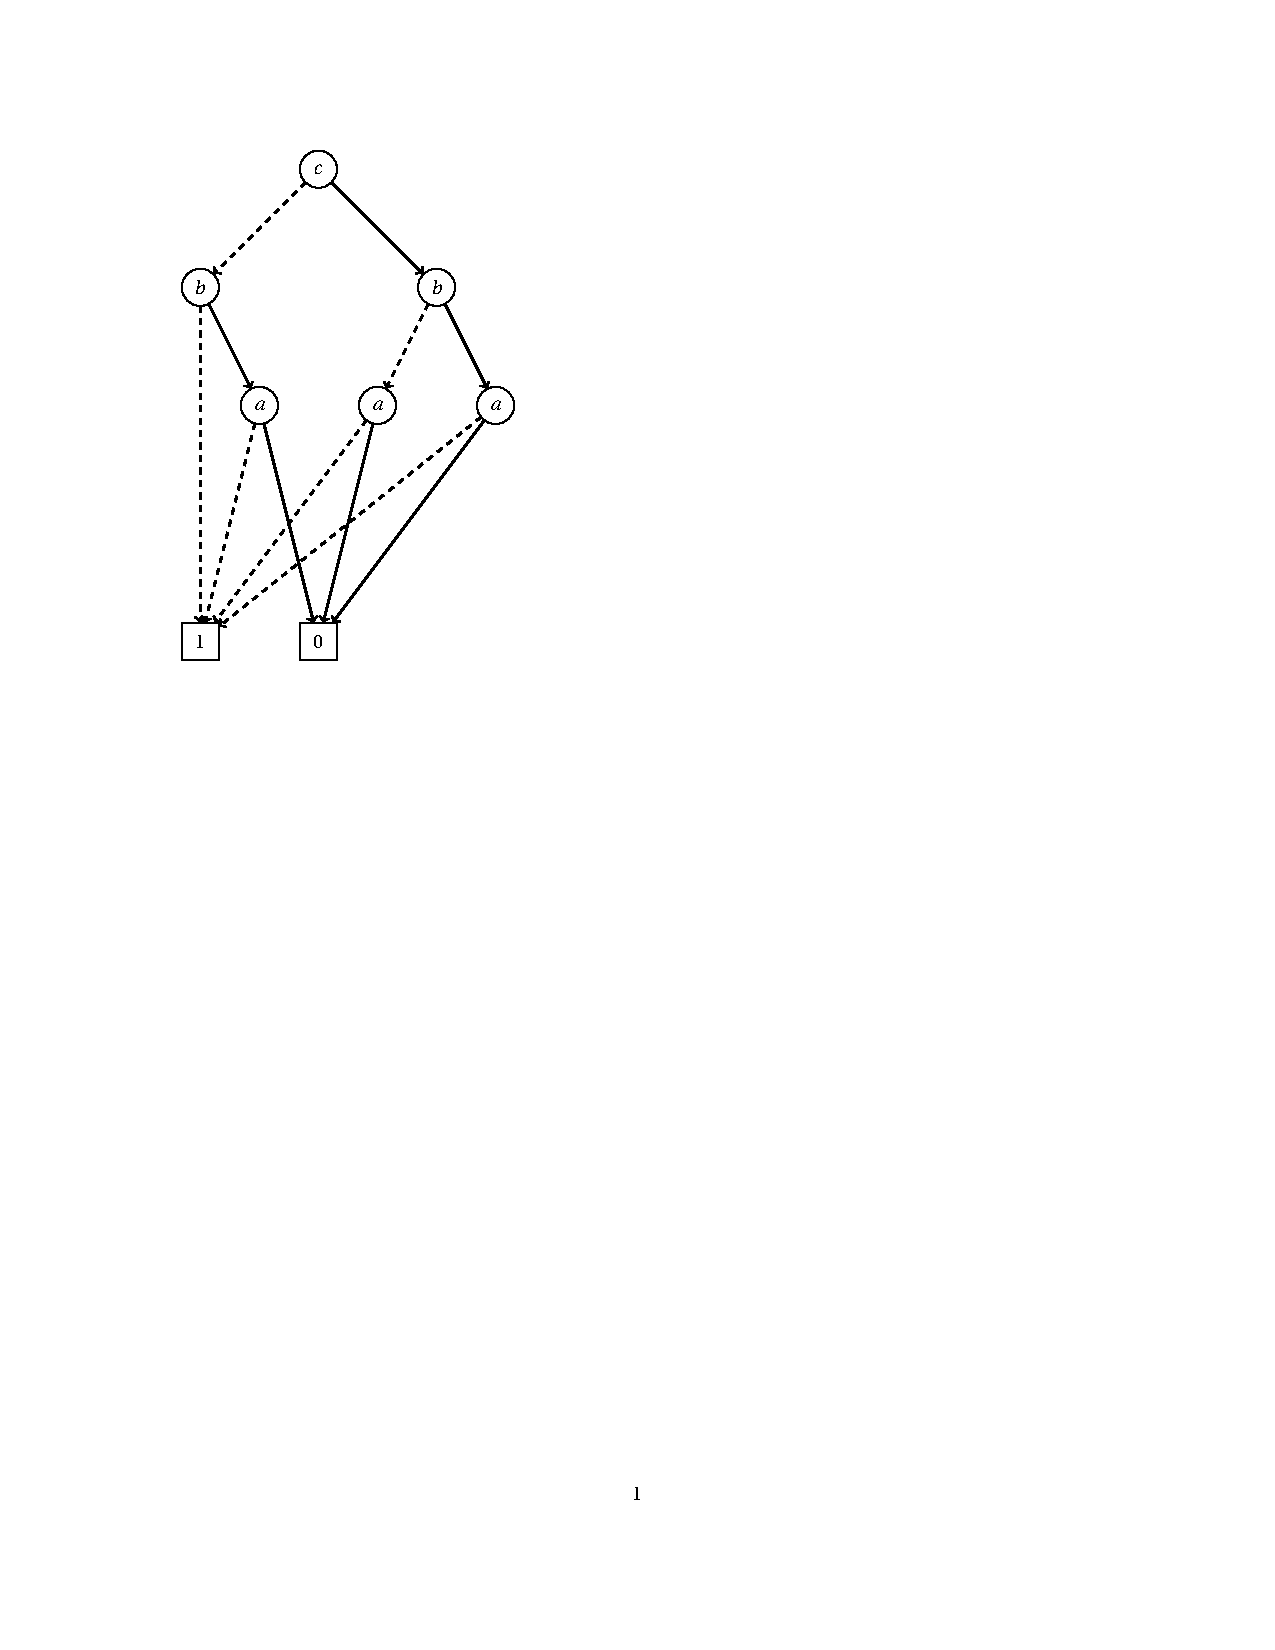
\includegraphics[
                trim=1cm 15.5cm 12cm 2cm,  clip=true]{ROBDD_bad.pdf}}
                \label{fig:ROBDDs:C}}  
            \end{tabular}
    \caption{exemplo do uso de ROBDDs para representar o espaço de 
        busca corrente durante a execução do algoritmo {\tt UCS}.} 
  \label{fig:ROBDDs} 
\end{figure}
\end{frame}

\section{UCSR2 e UCSR3}
\begin{frame}{UCSR2 e UCSR3}
    \begin{itemize}
        \item{Ambos algoritmos possuem dinâmicas semelhantes ao UCS}.
        \item{Acham mais facilmente um elemento minimal ou maximal do
            espaço de busca}
        \item{Possuem consumo de tempo maior do que o UCS por conta 
            das operações de atualização da ROBDD.}
    \end{itemize}
\end{frame}

\section{UCSR4, UCSR5 e UCSR6}
\begin{frame}{UCSR4, UCSR5 e UCSR6}
    \begin{itemize}
        \item{Esses algoritmos surgem da simplificação da DFS presente
            no UCS. Realiza-se agora um passeio tal que, dado $X$ do 
            espaço de busca, avalia-se todo $Y$ adjacente e:}
            \begin{itemize}
                \item[i.] se $Y$ é adjacente superior (inferior) e tem
                    custo menor que $X$, restringimos o intervalo
                    $[\emptyset, X]$ ($[X, S]$) e passamos a avaliar 
                    $Y$;
                \item[ii.] se $Y$ é adjacente superior (inferior) e tem
                    custo maior que $X$, podemos restringir, ou não, 
                    como será discutido na próxima sessão, o intervalo 
                    $[Y, S]$ ($[\emptyset, Y]$);
                \item[iii.] se $Y$ é adjacente superior (inferior) e
                    tem custo igual a $X$ não fazemos nada;
                \item[iv.] paramos quando não houverem mais elementos 
                    adjacentes a $X$.
            \end{itemize}
        \item{Existe um trade-off entre os algoritmos UCSR5 e UCSR6.}
    \end{itemize}
\end{frame}

\section{Primeiros Resultados}
\begin{frame}{Primeiros Resultados}
    
\begin{table}[h] \begin{center}
\resizebox{\columnwidth}{!}{%
\begin{tabular}{@{}ccc ccc ccc ccc ccc ccc ccc ccc ccc cc@{}} \toprule
\multicolumn{2}{c}{Instância} & \multicolumn{7}{c}{Tempo (segundos)}\\
\cline{1-2} \cline{4-10} 
$|S|$ & $2^{|S|}$  &&  UCSR6 & UCSR5 & UCSR4 & UCSR3 & UCSR2 & UCS & ES    \\ \hline
 1 &       2 &&  0.00 & 0.00 & 0.00 & 0.00 & 0.00 & 0.00 & 0.00 & \\ 
 2 &       4 &&  0.00 & 0.00 & 0.00 & 0.00 & 0.00 & 0.00 & 0.00 & \\ 
 3 &       8 &&  0.00 & 0.00 & 0.00 & 0.00 & 0.00 & 0.00 & 0.00 & \\ 
 4 &      16 &&  0.01 & 0.01 & 0.01 & 0.01 & 0.01 & 0.01 & 0.00 & \\ 
 5 &      32 &&  0.01 & 0.01 & 0.01 & 0.01 & 0.01 & 0.01 & 0.01 & \\ 
 6 &      64 &&  0.01 & 0.01 & 0.01 & 0.01 & 0.01 & 0.01 & 0.01 & \\ 
 7 &     128 &&  0.01 & 0.01 & 0.01 & 0.01 & 0.02 & 0.02 & 0.01 & \\ 
 8 &     256 &&  0.02 & 0.02 & 0.02 & 0.02 & 0.03 & 0.03 & 0.02 & \\ 
 9 &     512 &&  0.04 & 0.05 & 0.04 & 0.04 & 0.06 & 0.07 & 0.04 & \\ 
10 &    1024 &&  0.08 & 0.09 & 0.08 & 0.08 & 0.13 & 0.13 & 0.09 & \\ 
11 &    2048 &&  0.14 & 0.15 & 0.14 & 0.16 & 0.27 & 0.27 & 0.18 & \\ 
12 &    4096 &&  0.44 & 0.47 & 0.44 & 0.61 & 0.99 & 0.71 & 0.36 & \\ 
13 &    8192 &&  0.70 & 0.74 & 0.75 & 1.25 & 2.03 & 1.44 & 0.73 & \\ 
14 &   16384 &&  2.42 & 2.37 & 2.47 & 4.60 & 6.90 & 4.82 & 1.52 & \\ 
15 &   32768 &&  3.27 & 3.23 & 3.17 & 6.94 & 11.07 & 7.06 & 3.11 & \\ 
16 &   65536 &&  27.11 & 25.75 & 26.73 & 57.83 & 83.44 & 44.56 & 6.46 & \\ 
17 &  131072 &&  61.17 & 56.54 & 56.64 & 142.34 & 174.26 & 108.07 & 13.49 & \\ 
18 &  262144 &&  293.86 & 262.42 & 273.24 & 699.01 & 740.60 & 366.96 & 27.93 & \\ 
19 &  524288 &&  645.57 & 578.95 & 589.50 & 1335.98 & 1632.08 & 907.94 & 58.80 & \\ 
\bottomrule \end{tabular} 
}
\end{center} \end{table}
\end{frame}

\begin{frame}{Primeiros Resultados}
\begin{table}[ht] \begin{center} 
\resizebox{\columnwidth}{!}{%
\begin{tabular}{@{}ccc ccc ccc ccc ccc ccc ccc ccc ccc cc@{}} \toprule
\multicolumn{2}{c}{Instância} & \multicolumn{7}{c}{Número de chamadas da função custo}\\
\cline{1-2}\cline{4-10} 
$|S|$ & $2^{|S|}$  && UCSR6 & UCSR5 & UCSR4 & UCSR3 & UCSR2 & UCS & ES \\ \hline
 1 &       2 &&  2.00 &  2.00 &  2.00 &  2.00 &  2.00 &  2.00 & 2 & \\ 
 2 &       4 &&  3.80 &  4.00 &  4.20 &  3.80 &  3.80 &  3.90 & 4 & \\ 
 3 &       8 &&  6.50 &  7.30 &  7.30 &  6.50 &  6.45 &  6.50 & 8 & \\ 
 4 &      16 &&  12.85 & 13.70 & 14.05 & 12.80 & 12.60 & 12.85 & 16 & \\ 
 5 &      32 &&  19.95 & 21.30 & 21.40 & 21.00 & 19.75 & 19.20 & 32 & \\ 
 6 &      64 &&  31.25 & 33.40 & 33.35 & 32.50 & 31.25 & 36.40 & 64 & \\ 
 7 &     128 &&  50.70 & 58.15 & 62.15 & 53.90 & 50.85 & 56.00 & 128 & \\ 
 8 &     256 &&  86.50 & 94.85 & 101.70 & 92.90 & 89.60 & 94.45 & 256 & \\ 
 9 &     512 &&  170.60 & 191.00 & 203.60 & 179.75 & 171.25 & 174.50 & 512 & \\ 
10 &    1024 &&  273.75 & 322.25 & 336.75 & 286.10 & 272.70 & 280.05 & 1024 & \\ 
11 &    2048 &&  425.15 & 500.40 & 532.10 & 440.80 & 430.90 & 441.20 & 2048 & \\ 
12 &    4096 &&  1119.00 & 1271.80 & 1362.35 & 1121.55 & 1096.65 & 1077.45 & 4096 & \\ 
13 &    8192 &&  1437.10 & 1637.35 & 1692.30 & 1524.75 & 1437.00 & 1412.90 & 8192 & \\ 
14 &   16384 &&  2710.20 & 3203.10 & 3317.95 & 2874.50 & 2791.55 & 2702.25 & 16384 & \\ 
15 &   32768 &&  3181.60 & 3522.90 & 3764.50 & 3251.45 & 3147.50 & 3088.65 & 32768 & \\ 
16 &   65536 &&  9637.20 & 11544.65 & 11603.25 & 9923.35 & 9613.25 & 9380.85 & 65536 & \\ 
17 &  131072 &&  10327.90 & 12122.05 & 12301.70 & 10680.95 & 10370.95 & 9962.50 & 131072 & \\ 
18 &  262144 &&  21838.55 & 25847.15 & 26551.45 & 22676.30 & 21562.70 & 20920.90 & 262144 & \\ 
19 &  524288 &&  27931.55 & 32460.70 & 34011.60 & 28795.00 & 27823.70 & 27099.90 & 524288 & \\ 
\bottomrule \end{tabular}
}
\end{center} \end{table}
\end{frame}

\section{Reordenação do ROBDD}
\begin{frame}{Reordenação do ROBDD}
    \begin{itemize}
        \item{Achar a ordenação ótima é NP-difícil \cite{bollig}.}
        \item{Implementação de um algoritmo genético que procura por
            uma ordenação sub-ótima, o UCSR7.}

\begin{table}[ht] \begin{center}
\resizebox{200pt}{!}{%
\begin{tabular}{c c c c c c c} \toprule
\multicolumn{2}{c}{Instância} && \multicolumn{4}{c}{Tempo de execução em segundos}\\
\cline{1-2} \cline{4-7} \\
$|S|$ & $2^{|S|}$  && UCSR7 & UCSR6 & UCSR5 & ES \\ \hline
 1 &       2 & & 0.00 & 0.00 & 0.00 & 0.00 \\ 
 2 &       4 & & 0.00 & 0.00 & 0.00 & 0.00 \\ 
 3 &       8 & & 0.01 & 0.00 & 0.00 & 0.00 \\ 
 4 &      16 & & 0.03 & 0.00 & 0.00 & 0.00 \\ 
 5 &      32 & & 0.11 & 0.01 & 0.01 & 0.00 \\ 
 6 &      64 & & 0.29 & 0.01 & 0.01 & 0.01 \\
 7 &     128 & & 1.12 & 0.01 & 0.01 & 0.01 \\ 
 8 &     256 & & 1.87 & 0.02 & 0.02 & 0.02 \\ 
 9 &     512 & & 10.51 & 0.04 & 0.05 &0.04 \\ 
10 &    1024 & & 14.49 & 0.06 & 0.06 &0.08 \\
\bottomrule \end{tabular}
}
\end{center} \end{table}        
\end{itemize}
\end{frame}

\section{Atividades Futuras}
\begin{frame}{Atividades Futuras}
    \begin{itemize}
        \item{Estudar o momento em que devemos reordenar o ROBDD.}
        \item{Estudar como achar uma ordenação sub-ótima do ROBDD
            de maneira mais eficiente.}
        \item{Testar os algoritmos elaborados em instâncias reais.}
    \end{itemize}
\end{frame}

\section{Referências}
\begin{frame}{Referências}
\begin{thebibliography}{9} \label{sec:referencias}
\addcontentsline{toc}{section}{Referências}
\bibitem{msreis thesis}
Reis, Marcelo S. ``Minimization of decomposable in U-shaped curves 
functions defined on poset chains–algorithms and applications." PhD
thesis, Institute of Mathematics and Statistics, University of São 
Paulo, Brazil, (2012).
\bibitem{bryant}
Bryant, Randal E. ``Graph-based algorithms for boolean function
manipulation." IEEE Transactions on Computers, 100.8 (1986): 677-691.
\bibitem{bollig}
Bollig, Beate and Wegener, Ingo. ``Improving the variable ordering of
OBDDs is NP-complete." IEEE Transactions on Computers, 45.9 (1996):
993--1002.



\end{thebibliography}
\end{frame}

\end{document}

